\documentclass[8pt,executivepaper]{article}
\usepackage[utf8]{inputenc}
\usepackage[spanish]{babel}
\usepackage{amsmath}
\usepackage{amsfonts}
\usepackage{amssymb}
\usepackage{graphics}
\usepackage{graphicx}
\usepackage[left=1cm,right=1cm,top=2cm,bottom=2cm]{geometry}
\usepackage{imakeidx}
\makeindex[columns=3, title=Alphabetical Index, intoc]
\usepackage{listings}
\usepackage{xcolor}
\usepackage{multicol}
\usepackage{changepage}
\usepackage{float}
\usepackage{cite}
\usepackage{url}
\usepackage{hyperref}
\usepackage{pdfpages}
\definecolor{codegreen}{rgb}{0,0.6,0}
\definecolor{codegray}{rgb}{0.5,0.5,0.5}
\definecolor{codepurple}{rgb}{0.58,0,0.82}
\definecolor{backcolour}{rgb}{0.95,0.95,0.92}
\lstdefinestyle{mystyle}{
    backgroundcolor=\color{backcolour},
    commentstyle=\color{codegreen},
    keywordstyle=\color{magenta},
    numberstyle=\tiny\color{codegray},
    stringstyle=\color{codepurple},
    basicstyle=\ttfamily\footnotesize,
    breakatwhitespace=false,
    breaklines=true,
    captionpos=b,
    keepspaces=true,
    numbers=left,
    numbersep=5pt,
    showspaces=false,
    showstringspaces=false,
    showtabs=false,
    tabsize=3
}
\lstset{style=mystyle}
\author{González Pardo Adrian}
\date{Abril 2020}
\title{Reporte de practica 8}
\newcommand\tab[1][1cm]{\hspace*{#1}}
\begin{document}
\maketitle
\section{Código VHDL}
\lstinputlisting[language=VHDL]{vhdl/memPrograma.vhd}
\section{Test-Bench VHDL Código}
\lstinputlisting[language=VHDL]{tb/tbMemPrograma.vhd}
\textbf{Archivo de entrada (input.txt)}
\lstinputlisting{input.txt}
\textbf{Archivo de salida (output.txt)}
\lstinputlisting{output.txt}
\section{Simulaciones}
\begin{center}
  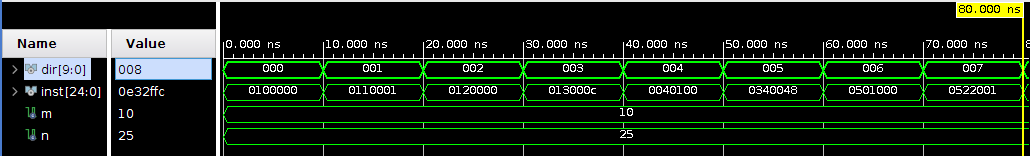
\includegraphics[scale=0.45]{imgs/uno.png}\\
  \textit{Figura 1: Primer parte del test-bench}\\
  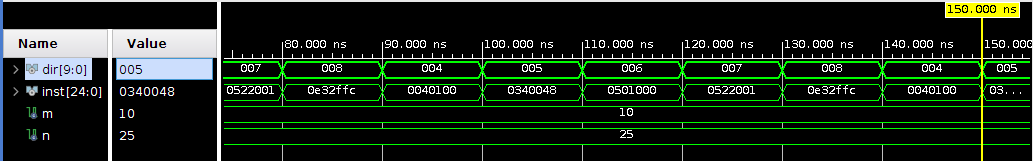
\includegraphics[scale=0.45]{imgs/dos.png}\\
  \textit{Figura 2: Segunda parte del test-bench}\\
  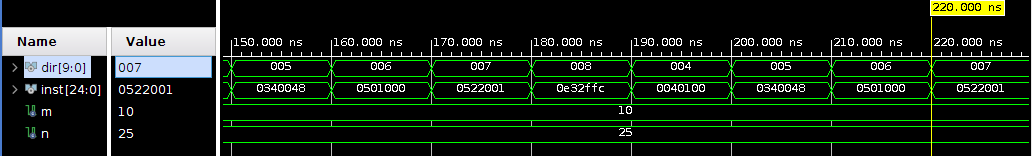
\includegraphics[scale=0.45]{imgs/tres.png}\\
  \textit{Figura 3: Tercer parte del test-bench}\\
  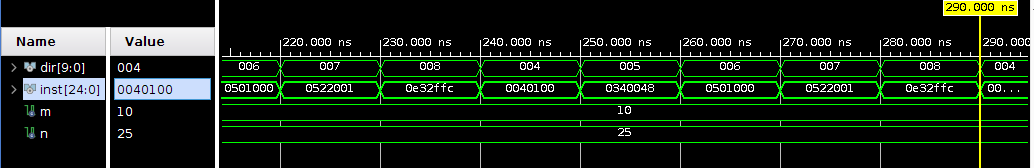
\includegraphics[scale=0.45]{imgs/cuatro.png}\\
  \textit{Figura 4: Cuarta parte del test-bench}\\
  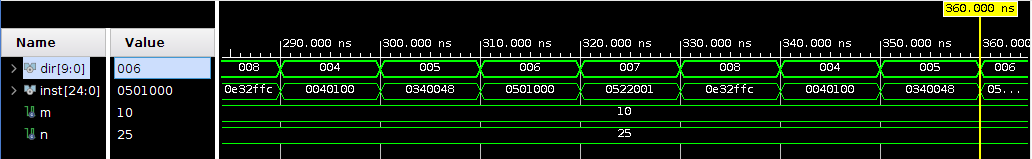
\includegraphics[scale=0.45]{imgs/cinco.png}\\
  \textit{Figura 5: Quinta parte del test-bench}\\
  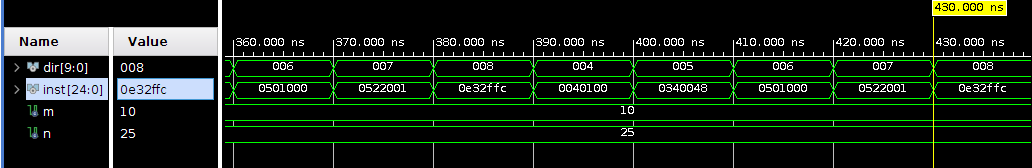
\includegraphics[scale=0.45]{imgs/seis.png}\\
  \textit{Figura 6: Sexta parte del test-bench}\\
  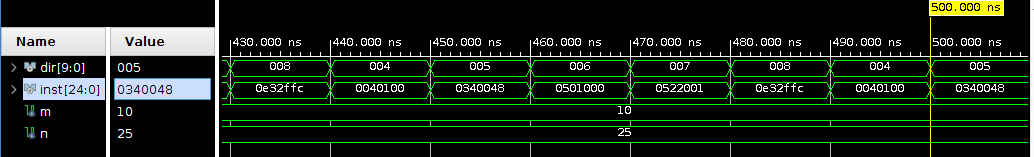
\includegraphics[scale=0.45]{imgs/siete.png}\\
  \textit{Figura 7: Septima parte del test-bench}\\
  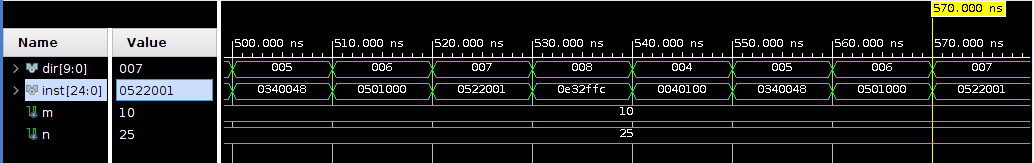
\includegraphics[scale=0.45]{imgs/ocho.png}\\
  \textit{Figura 8: Octava parte del test-bench}\\
  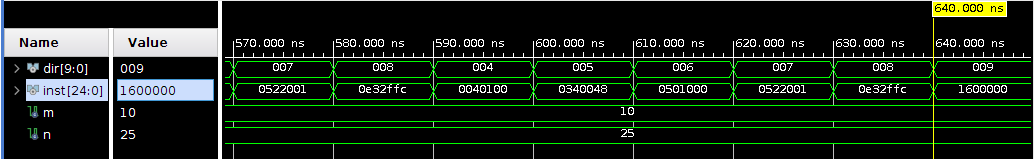
\includegraphics[scale=0.45]{imgs/nueve.png}\\
  \textit{Figura 9: Novena parte del test-bench}\\
  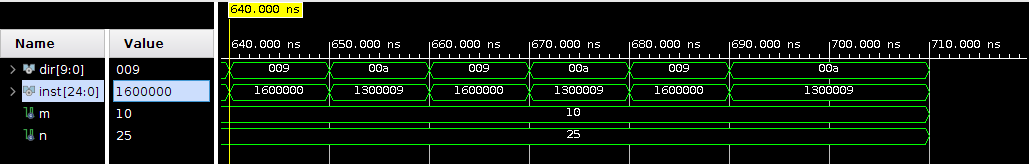
\includegraphics[scale=0.45]{imgs/diez.png}\\
  \textit{Figura 10: Decima parte del test-bench}

\end{center}
\section{Diagrama RTL}
\begin{center}
  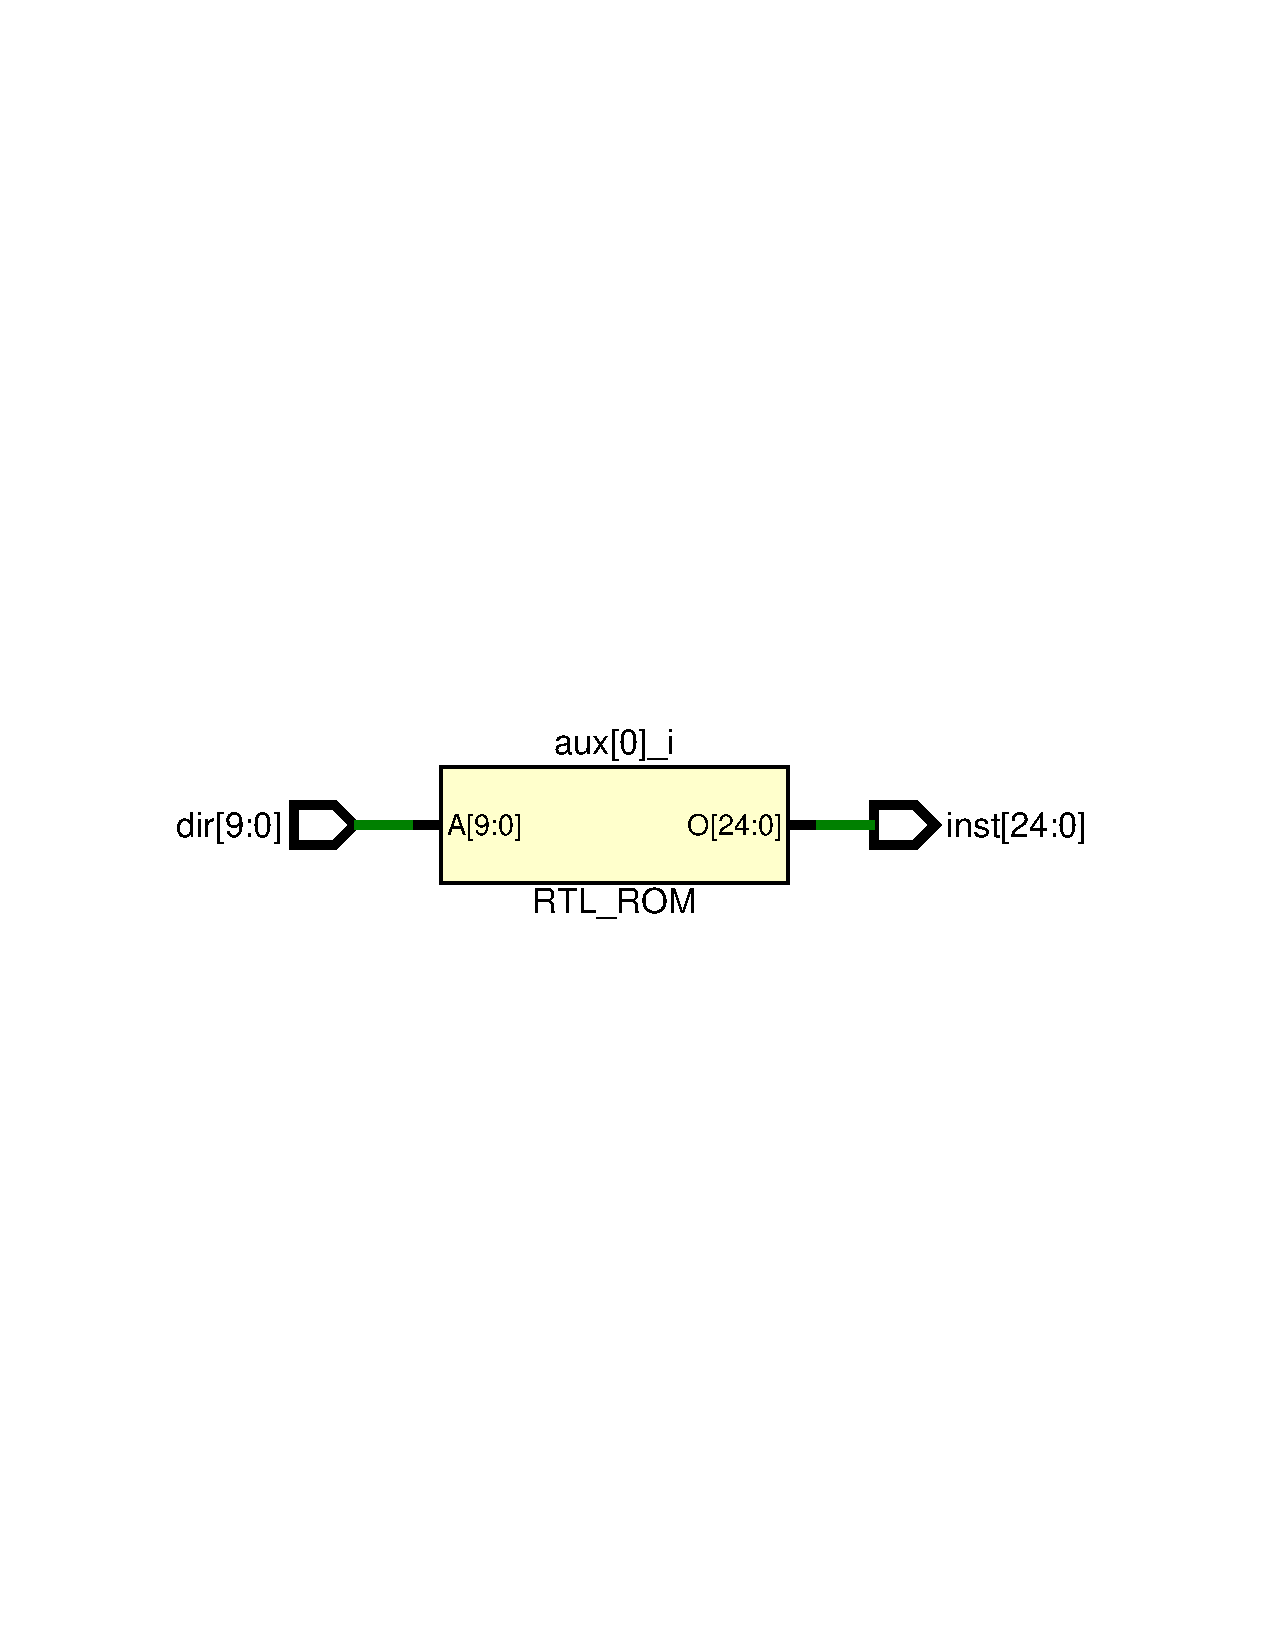
\includegraphics[scale=0.5]{sources/schematicRTL.pdf}
\end{center}
\end{document}
